\section{Auswertung}
\label{sec:Auswertung}

\subsection{Mittlere freie Weglänge}
\label{sec:mfw}
Zuerst wird die in der \autoref{sec:Theorie} erwähnte mittlere freie Weglänge
der Elektronen bestimmt, welche die Elektronen in dem Quecksilbergas zurücklegen,
wenn es zu einem Stoß kommt. Dazu werden die Temperaturen der Messungen 
in \autoref{eqn:6} eingesetzt. Die Resultate sind in \autoref{tab:10} 
aufgelistet.
\begin{table}[H]
  \centering
  \caption{Mittlere Freie Weglängen.}
  \label{tab:10}
  \begin{tblr}{
      colspec = {S S },
      row{1} = {guard, mode=math},}
         \toprule
         T/\, \unit{\kelvin} &\overline{\omega}/ \unit{\meter} \\
         \midrule
          296.15&\num{0.063e3}\\
          419.15&\num{7.02e-5}\\
          436.15&\num{3.75e-5}\\
          448.15&\num{2.42e-5}\\
          \bottomrule
  \end{tblr}
\end{table}
\noindent Es ist erkennbar, dass die Anzahl an Stößen proportional zur Temperatur 
ist. Bei Temperaturen im Bereich von $400\unit{\kelvin}$ bis $500 \unit{\kelvin}$ 
ist das Verhältnis der mittleren freien Weglänge zu dem Abstand von Kathode
zu Anode mit $a = 1 \unit{\centi\meter}$ sehr gering, was letztendlich den 
Franck-Hertz Versuch ermöglicht.

\subsection{Kontaktpotential}
In diesem Teil des Versuchs geht es darum das Kontaktpotential zu berechnen. 
In den Abbildungen \autoref{fig:10} und \autoref{fig:11} sind die Strom-
Gegenspannungs Messkurven abgebildet, welche mit dem XY-Schreiber 
aufgezeichnet wurden. Einersteits bei einer Temperatur von $296.15\unit{\kelvin}$
und einmal bei $419.15\unit{\kelvin}$.
\begin{figure}[H]
  \centering
  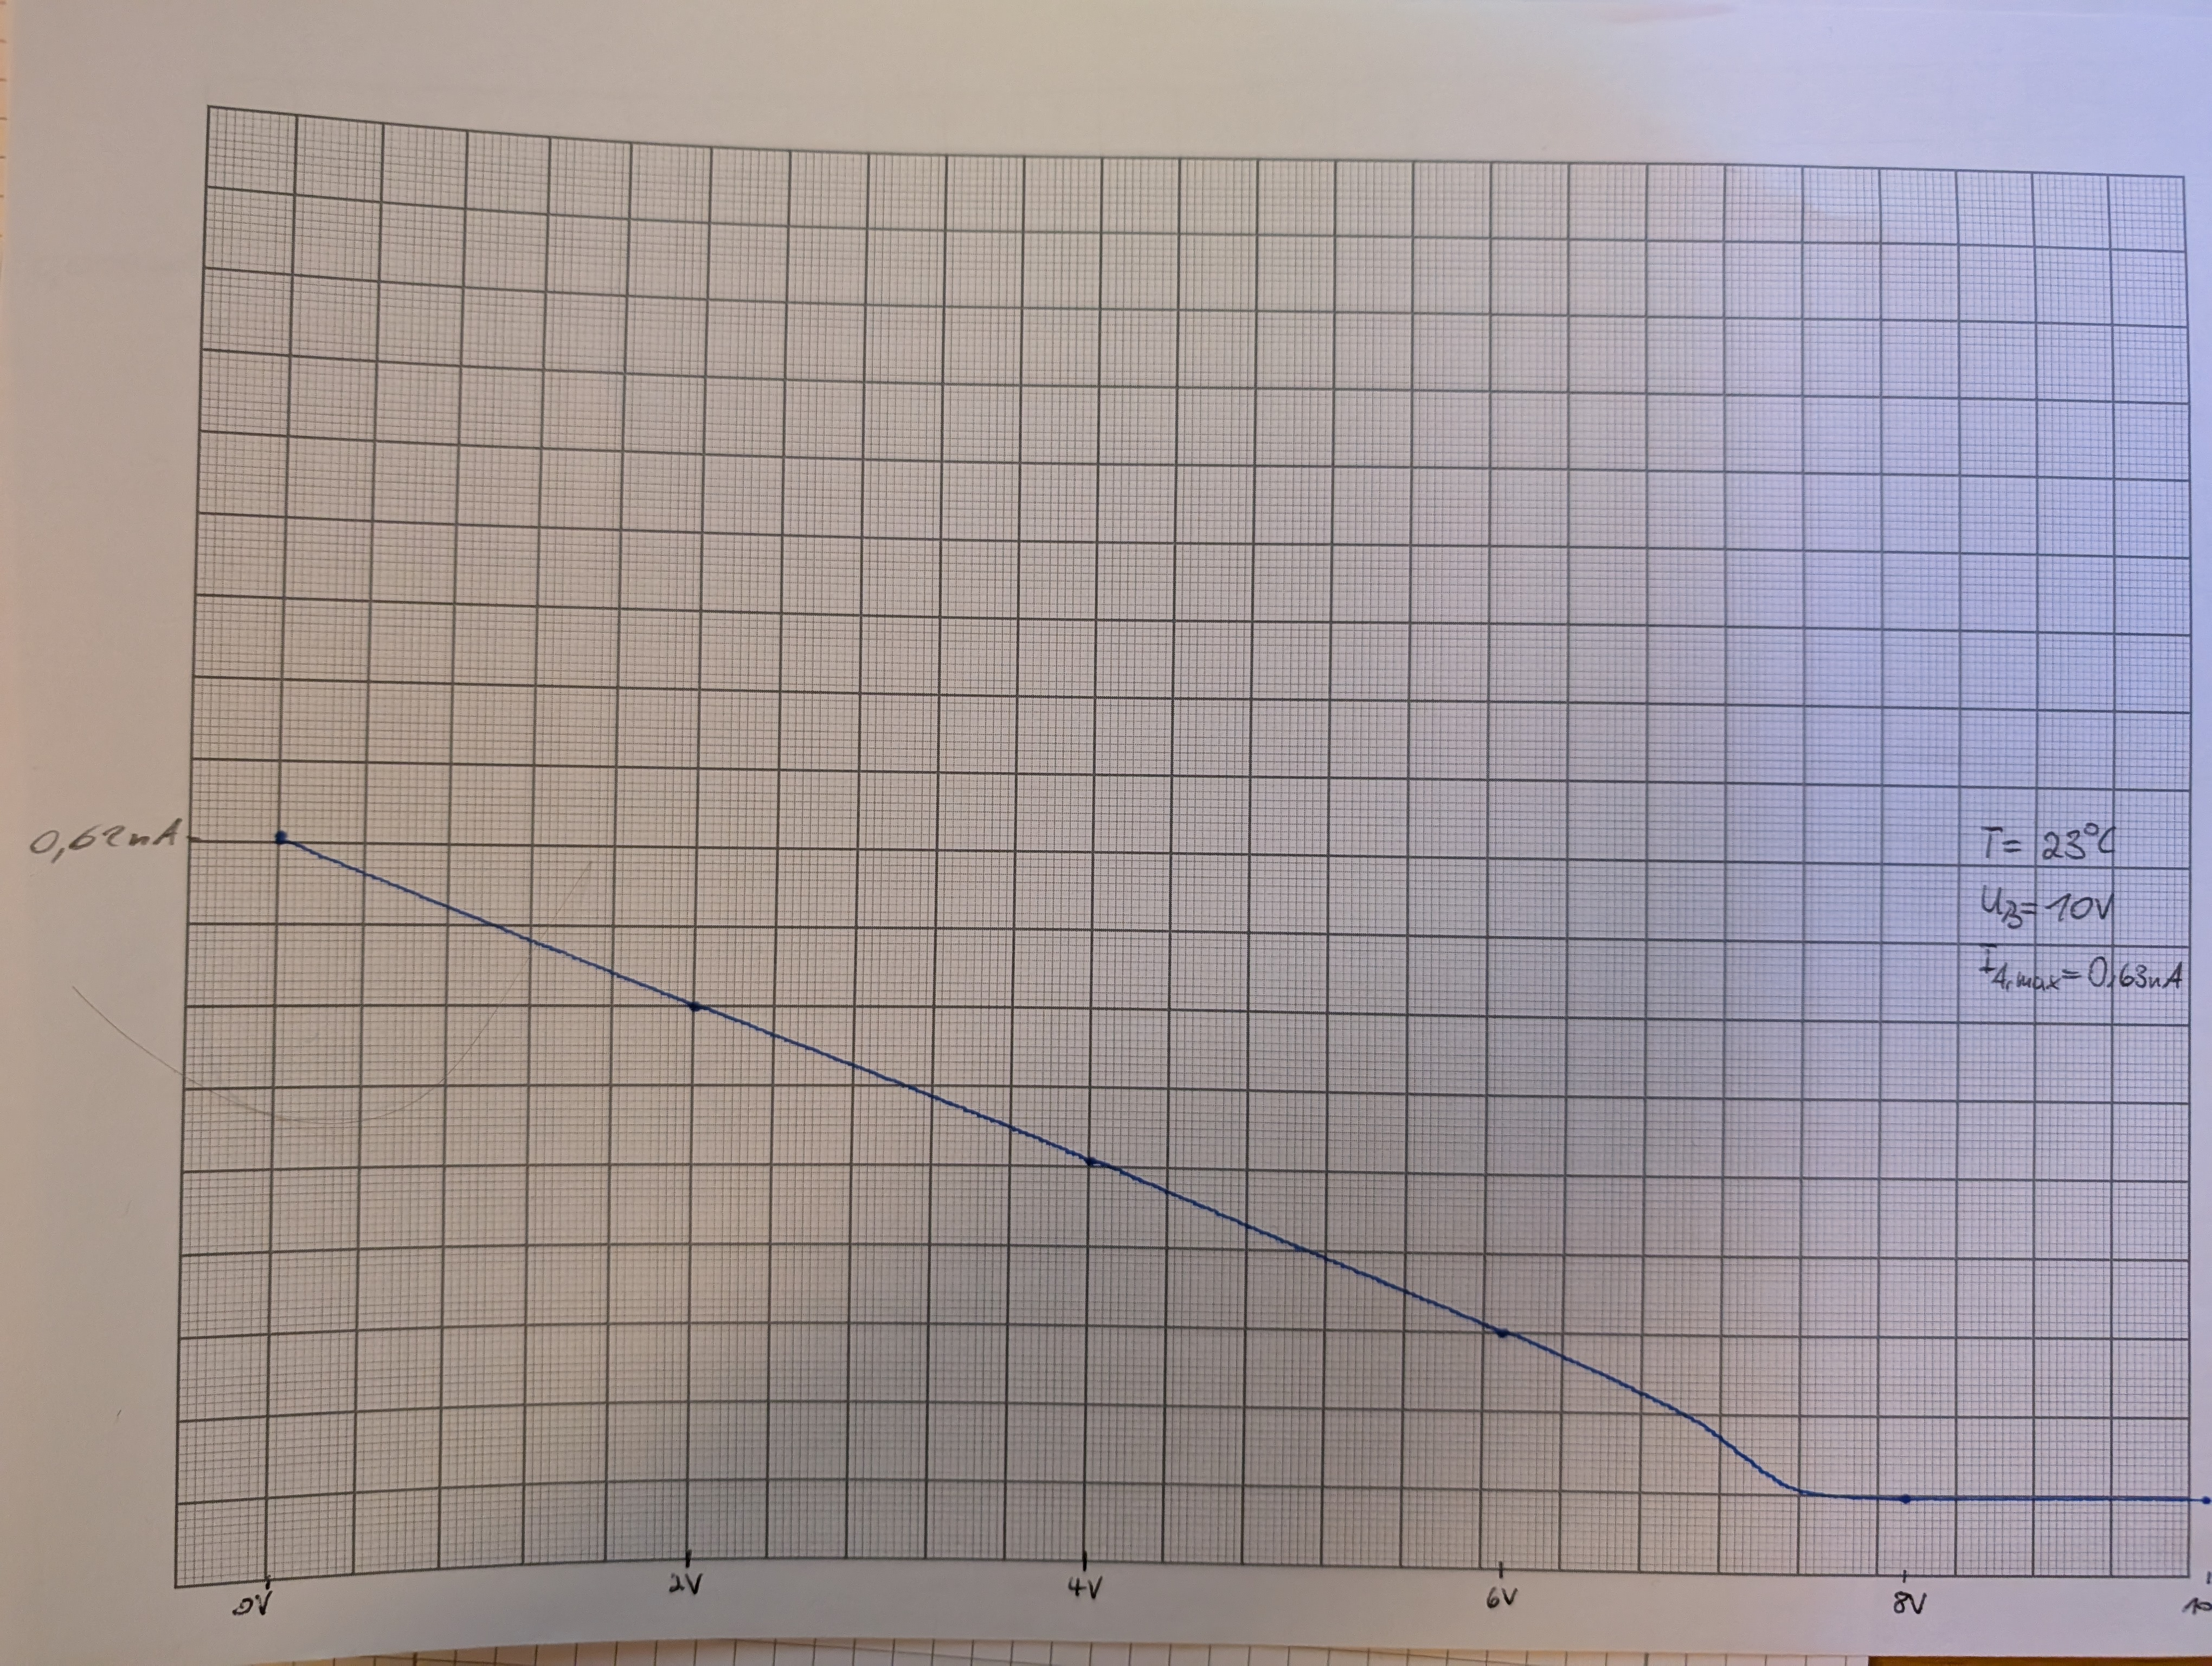
\includegraphics[width=0.7\linewidth]{Bilder/1.jpg}
  \caption{Strom-Spannungs Kurve bei 296.15\unit{\kelvin}}
  \label{fig:10}
\end{figure}

\begin{figure}[H]
  \centering
  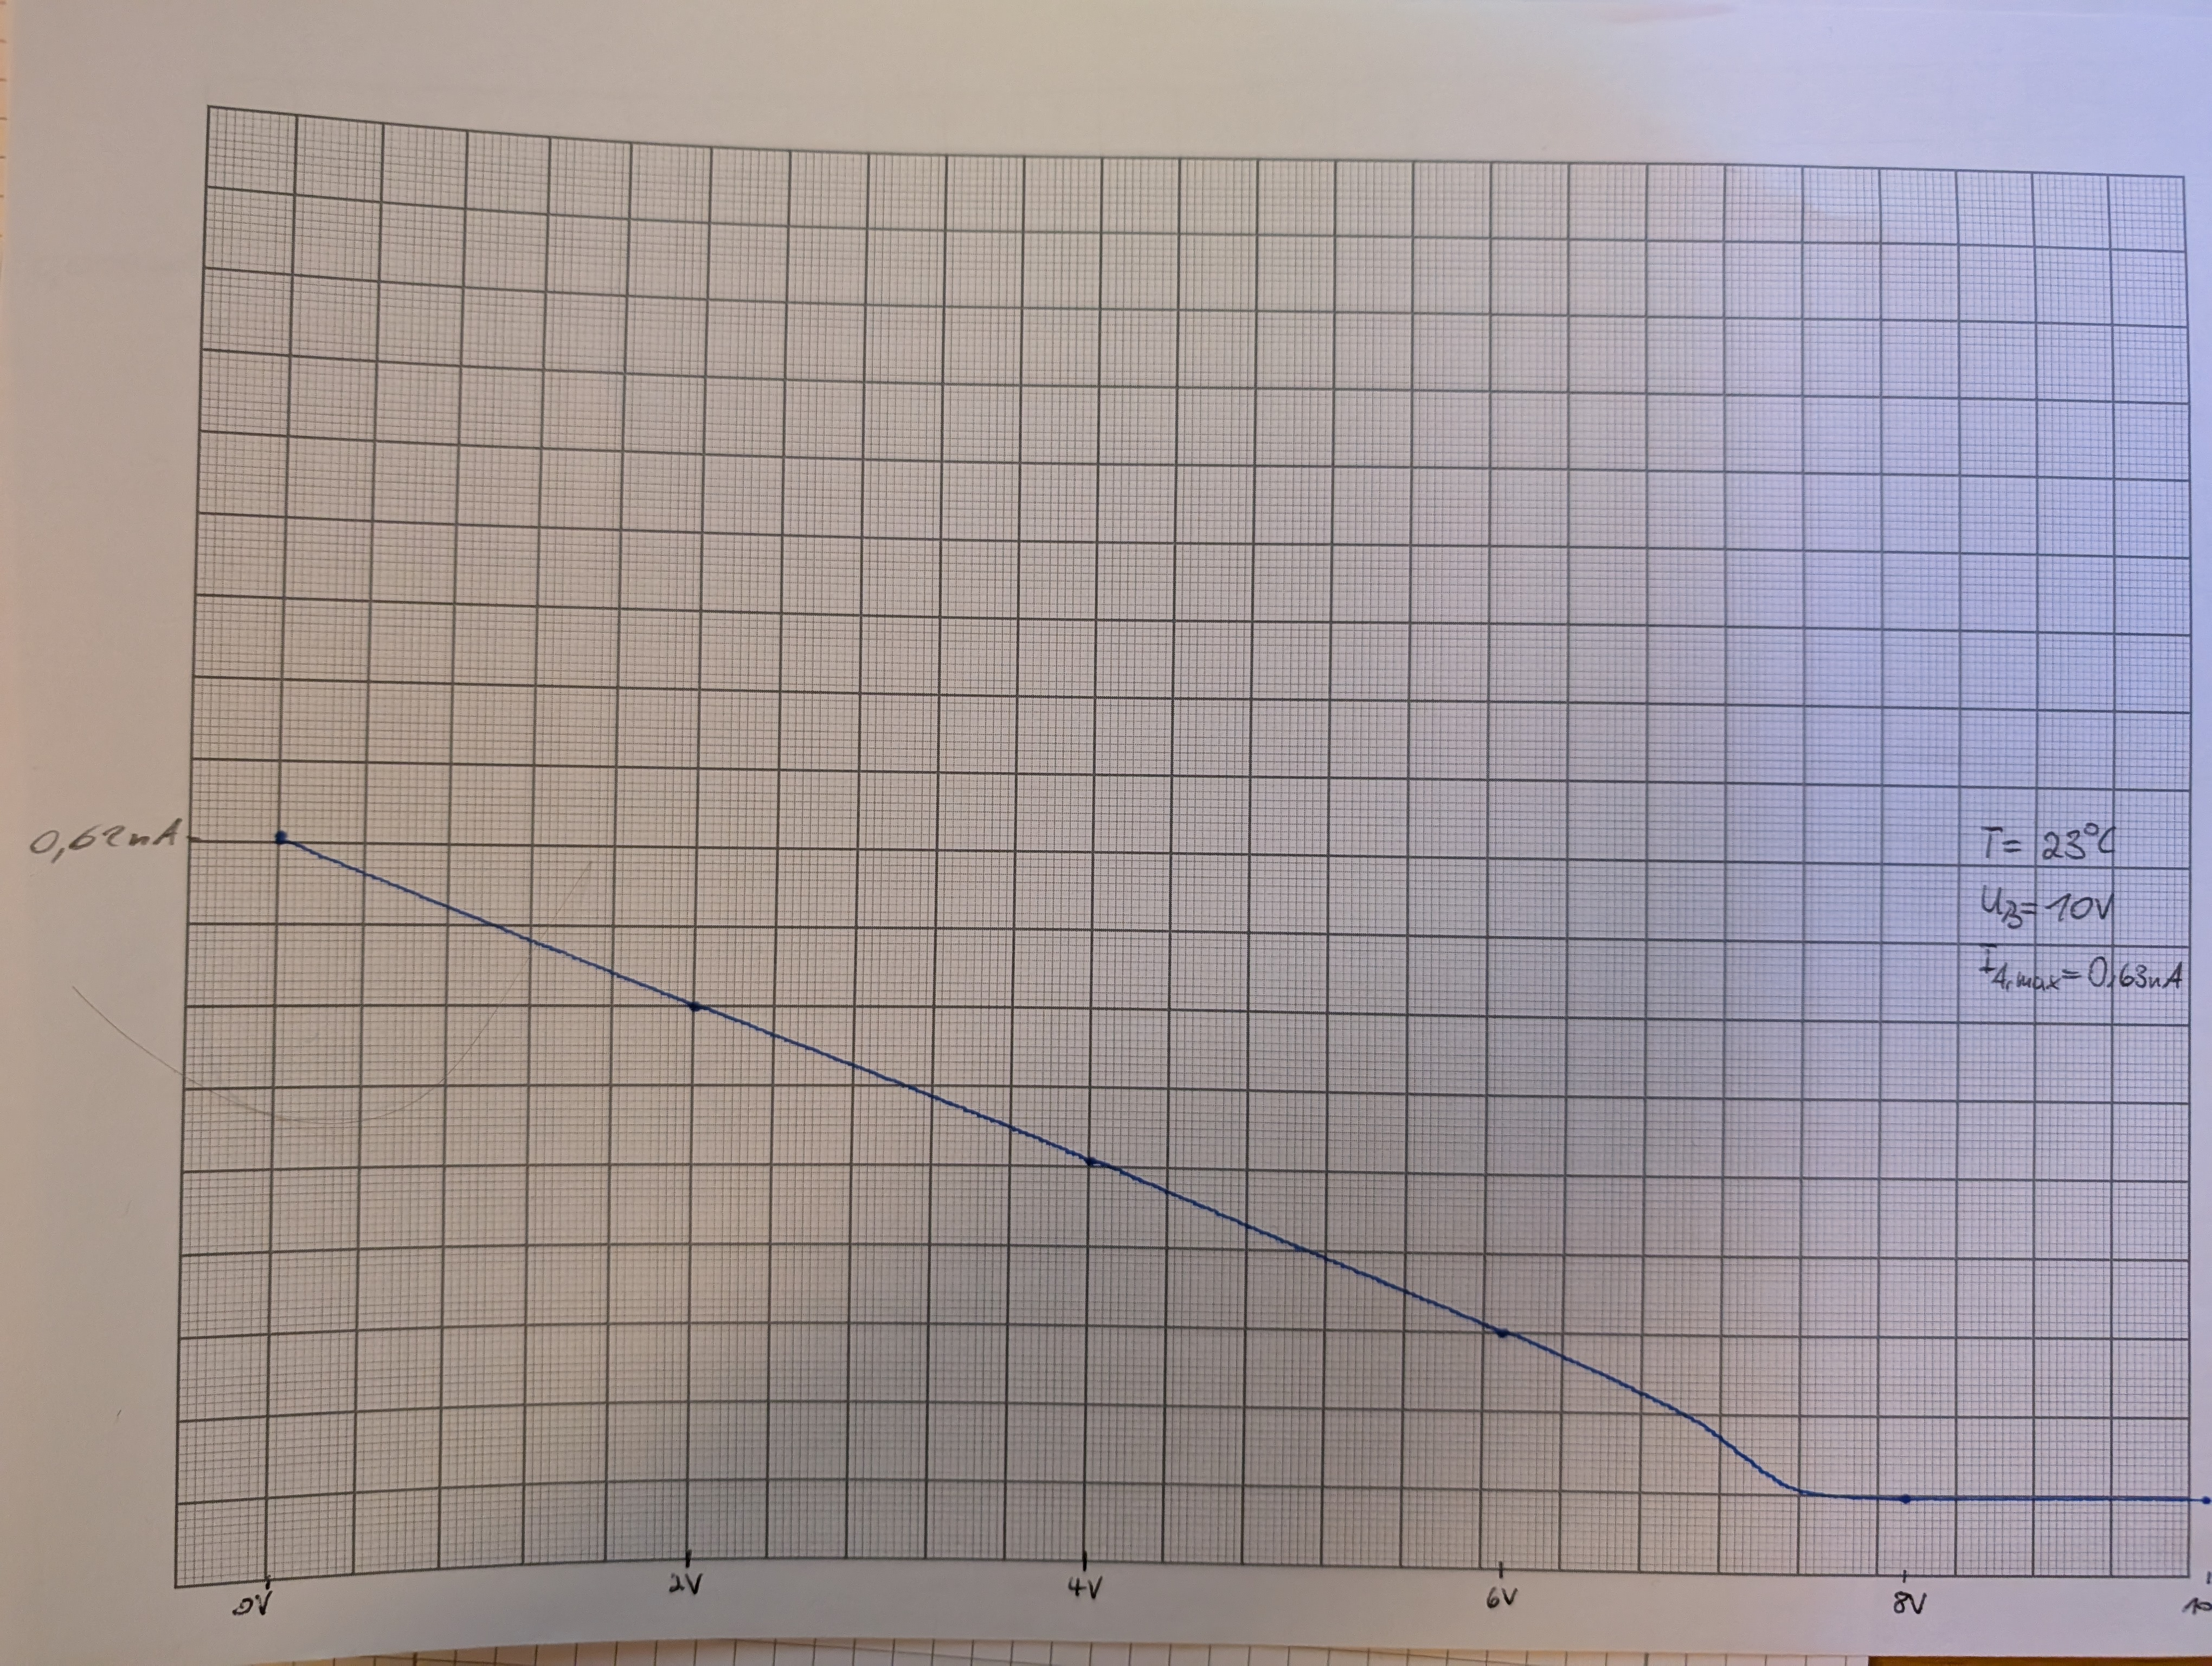
\includegraphics[width=0.7\linewidth]{Bilder/1.jpg}
  \caption{Strom-Spannungs Kurve bei 419.15\unit{\kelvin}}
  \label{fig:11}
\end{figure}

\noindent Aus diesen graphischen Daten muss der Differenzenquotient für bestimmte
Werte gebildet werden, um auf den Spannungspunkt mit der größten Steigung 
(Wendepunkt) zu schließen. Daraus lässt sich dann nach \autoref{eqn:5} 
das Kontaktpotential berechnen.

\noindent In \autoref{tab:11} sind die händisch ermittelten Differenzenquotienten
einiger Messpunkte für beide Tempeeraturen aufgetragen. Zusätzlich sind diese in
\autoref{fig:12} und \autoref{fig:13} graphisch dargestellt.
\begin{table}[H]
  \centering
  \caption{Differentiation der Messdaten.}
  \label{tab:11}
  \begin{tblr}{
      colspec = {S S | S S},
      row{1,2} = {guard, mode=math},}
         \toprule
         \SetCell[c=2]{c} T = 296.15\unit{\kelvin} &&  \SetCell[c=2]{c} T = 419.15\unit{\kelvin}  \\
          U / \unit{\volt}& I / U / \unit{\nano\ampere\per\volt} & U / \unit{\volt} & I / U / \unit{\nano\ampere\per\volt}\\
         \midrule
          2   & -0.073& 0   & 0       \\
          4   & -0.073& 0.25& -0.00594\\
          6   & -0.073& 0.5 & -0.00577\\
          6.5 & -0.085& 0.75& -0.0050\\
          6.6 & -0.089& 1   & -0.0050\\
          6.7 & -0.096& 1.25& -0.0047\\
          6.8 & -0.104& 1.5 & -0.0044\\
          6.9 & -0.106& 1.75& -0.0040\\
          7   & -0.111& 2   & -0.0036\\
          7.1 & -0.118& 2.25& -0.0028\\
          7.2 & -0.130& 2.5 & -0.0021\\
          7.3 & -0.139& 2.75& -0.0017\\
          7.4 & -0.124& 3   & -0.0007\\
          7.5 & -0.111& 3.25& -0.0002\\
          8   & 0     & 3.5 & 0      \\
          \bottomrule
  \end{tblr}
\end{table}
\begin{figure}[H]
  \centering
  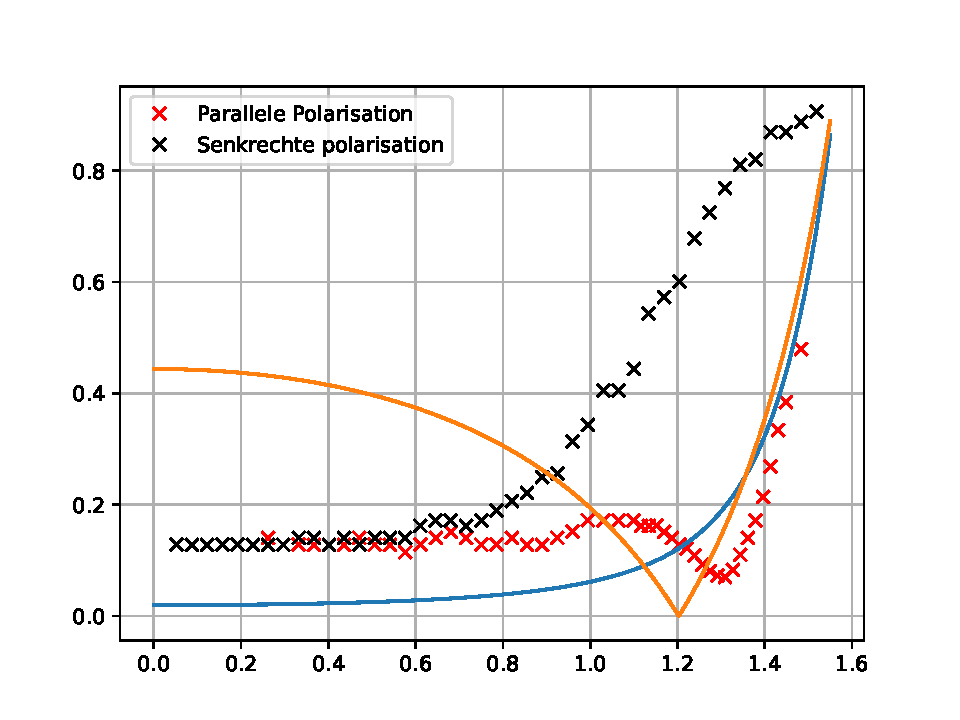
\includegraphics[width=\linewidth]{build/plot.pdf}
  \caption{Steigung der Kurve bei 296.15\unit{\kelvin}}
  \label{fig:12}
\end{figure}

\noindent Aus \autoref{fig:12} kann entnommen werden, dass die größte Steigung
(negative Steigung) am Punkt $U = 7.3\unit{\volt}$ vorliegt. Daraus berechnet
sich das Kontaktpotential zu
\begin{align*}
  U_\text{Kontakt} &= U_\text{B} - U_\text{B,eff} \\
                   &= 10 \unit{\volt} - 7.3 \unit{\volt} \\
                   &= 2.7 \unit{\volt}.
\end{align*}

\begin{figure}[H]
  \centering
  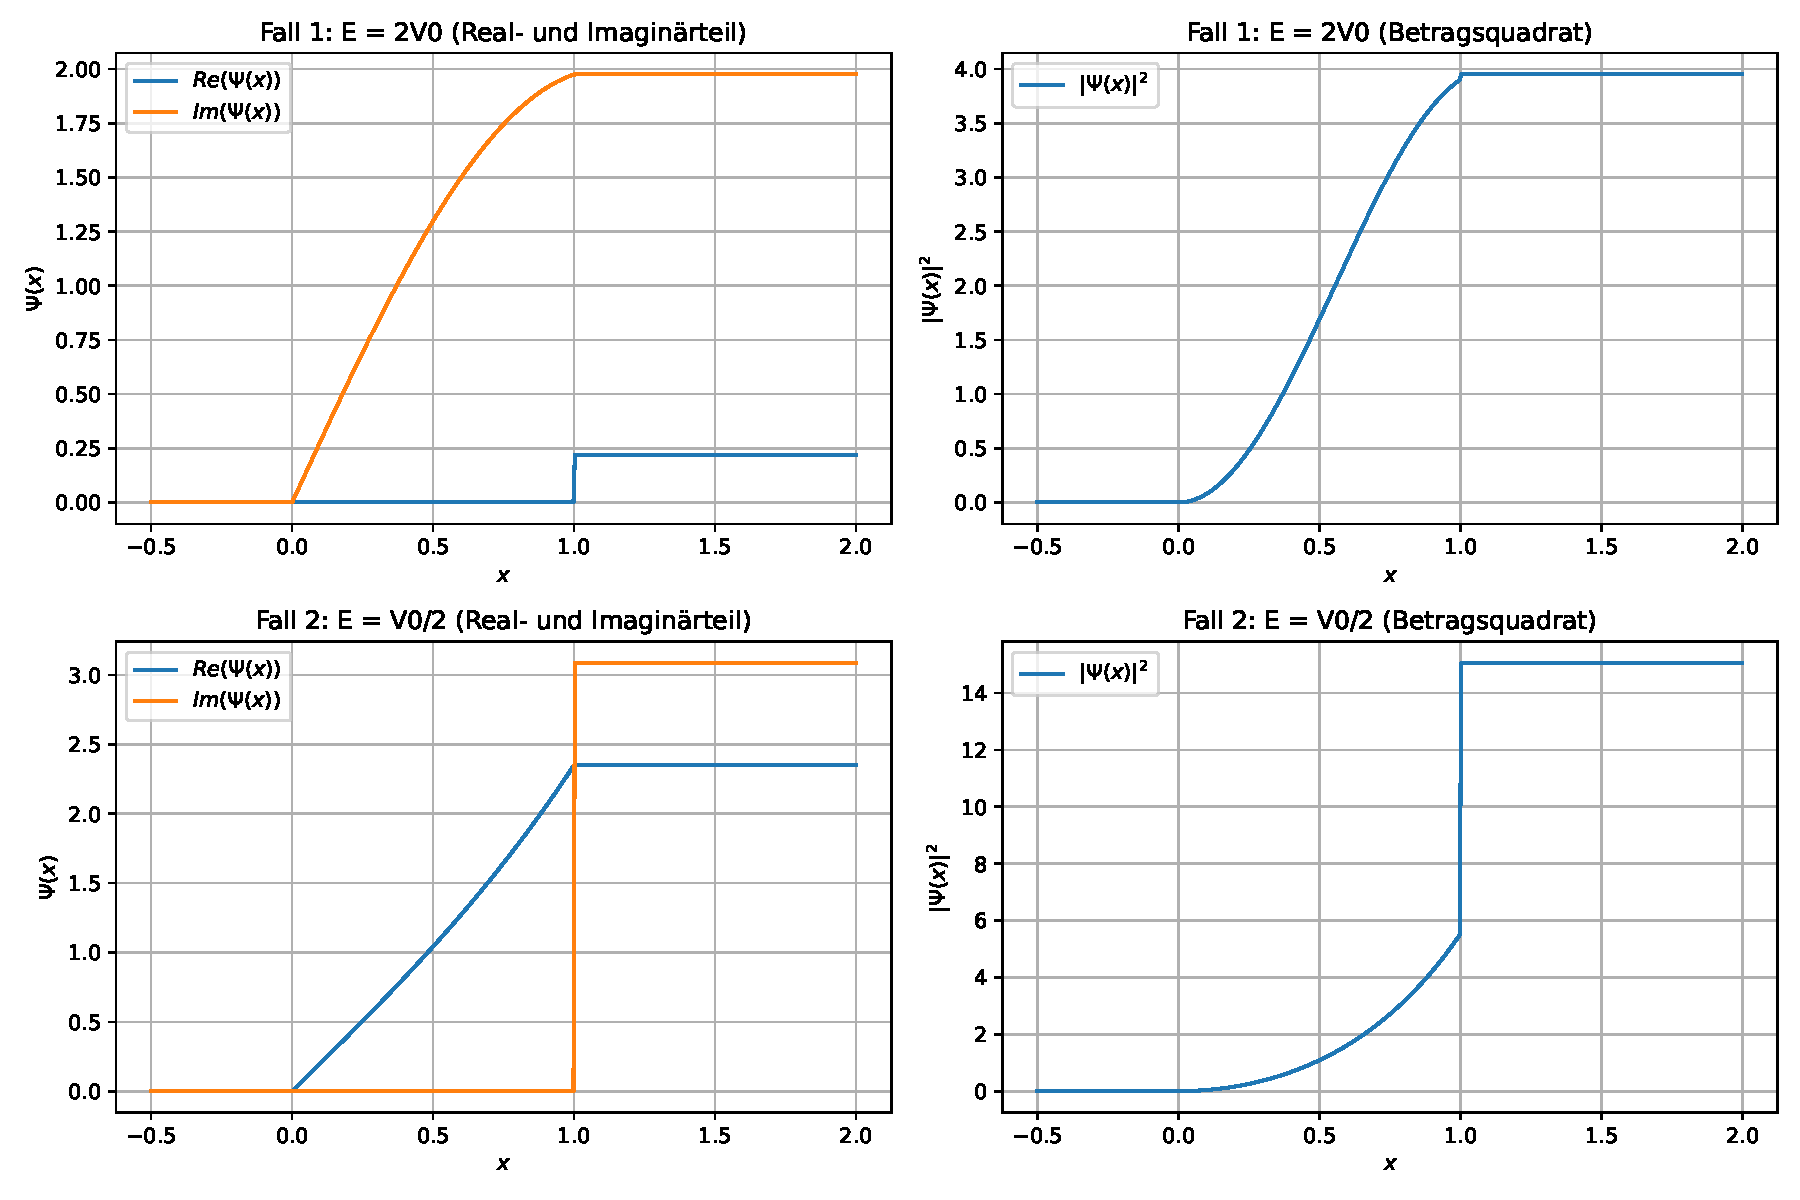
\includegraphics[width=\linewidth]{build/plot2.pdf}
  \caption{Steigung der Kurve bei 419.15\unit{\kelvin}}
  \label{fig:13}
\end{figure}

\subsection{Franck-Hertz Kurven}
Für die Auswertung der Franck-Hertz Kurven wurden $I_A$-Werte bei 
$436.15\unit{\kelvin}$ und $448.15\unit{\kelvin}$ aufgenommen. Diese sind in
\autoref{fig:14} abgebildet.
\begin{figure}[H]
  \centering
  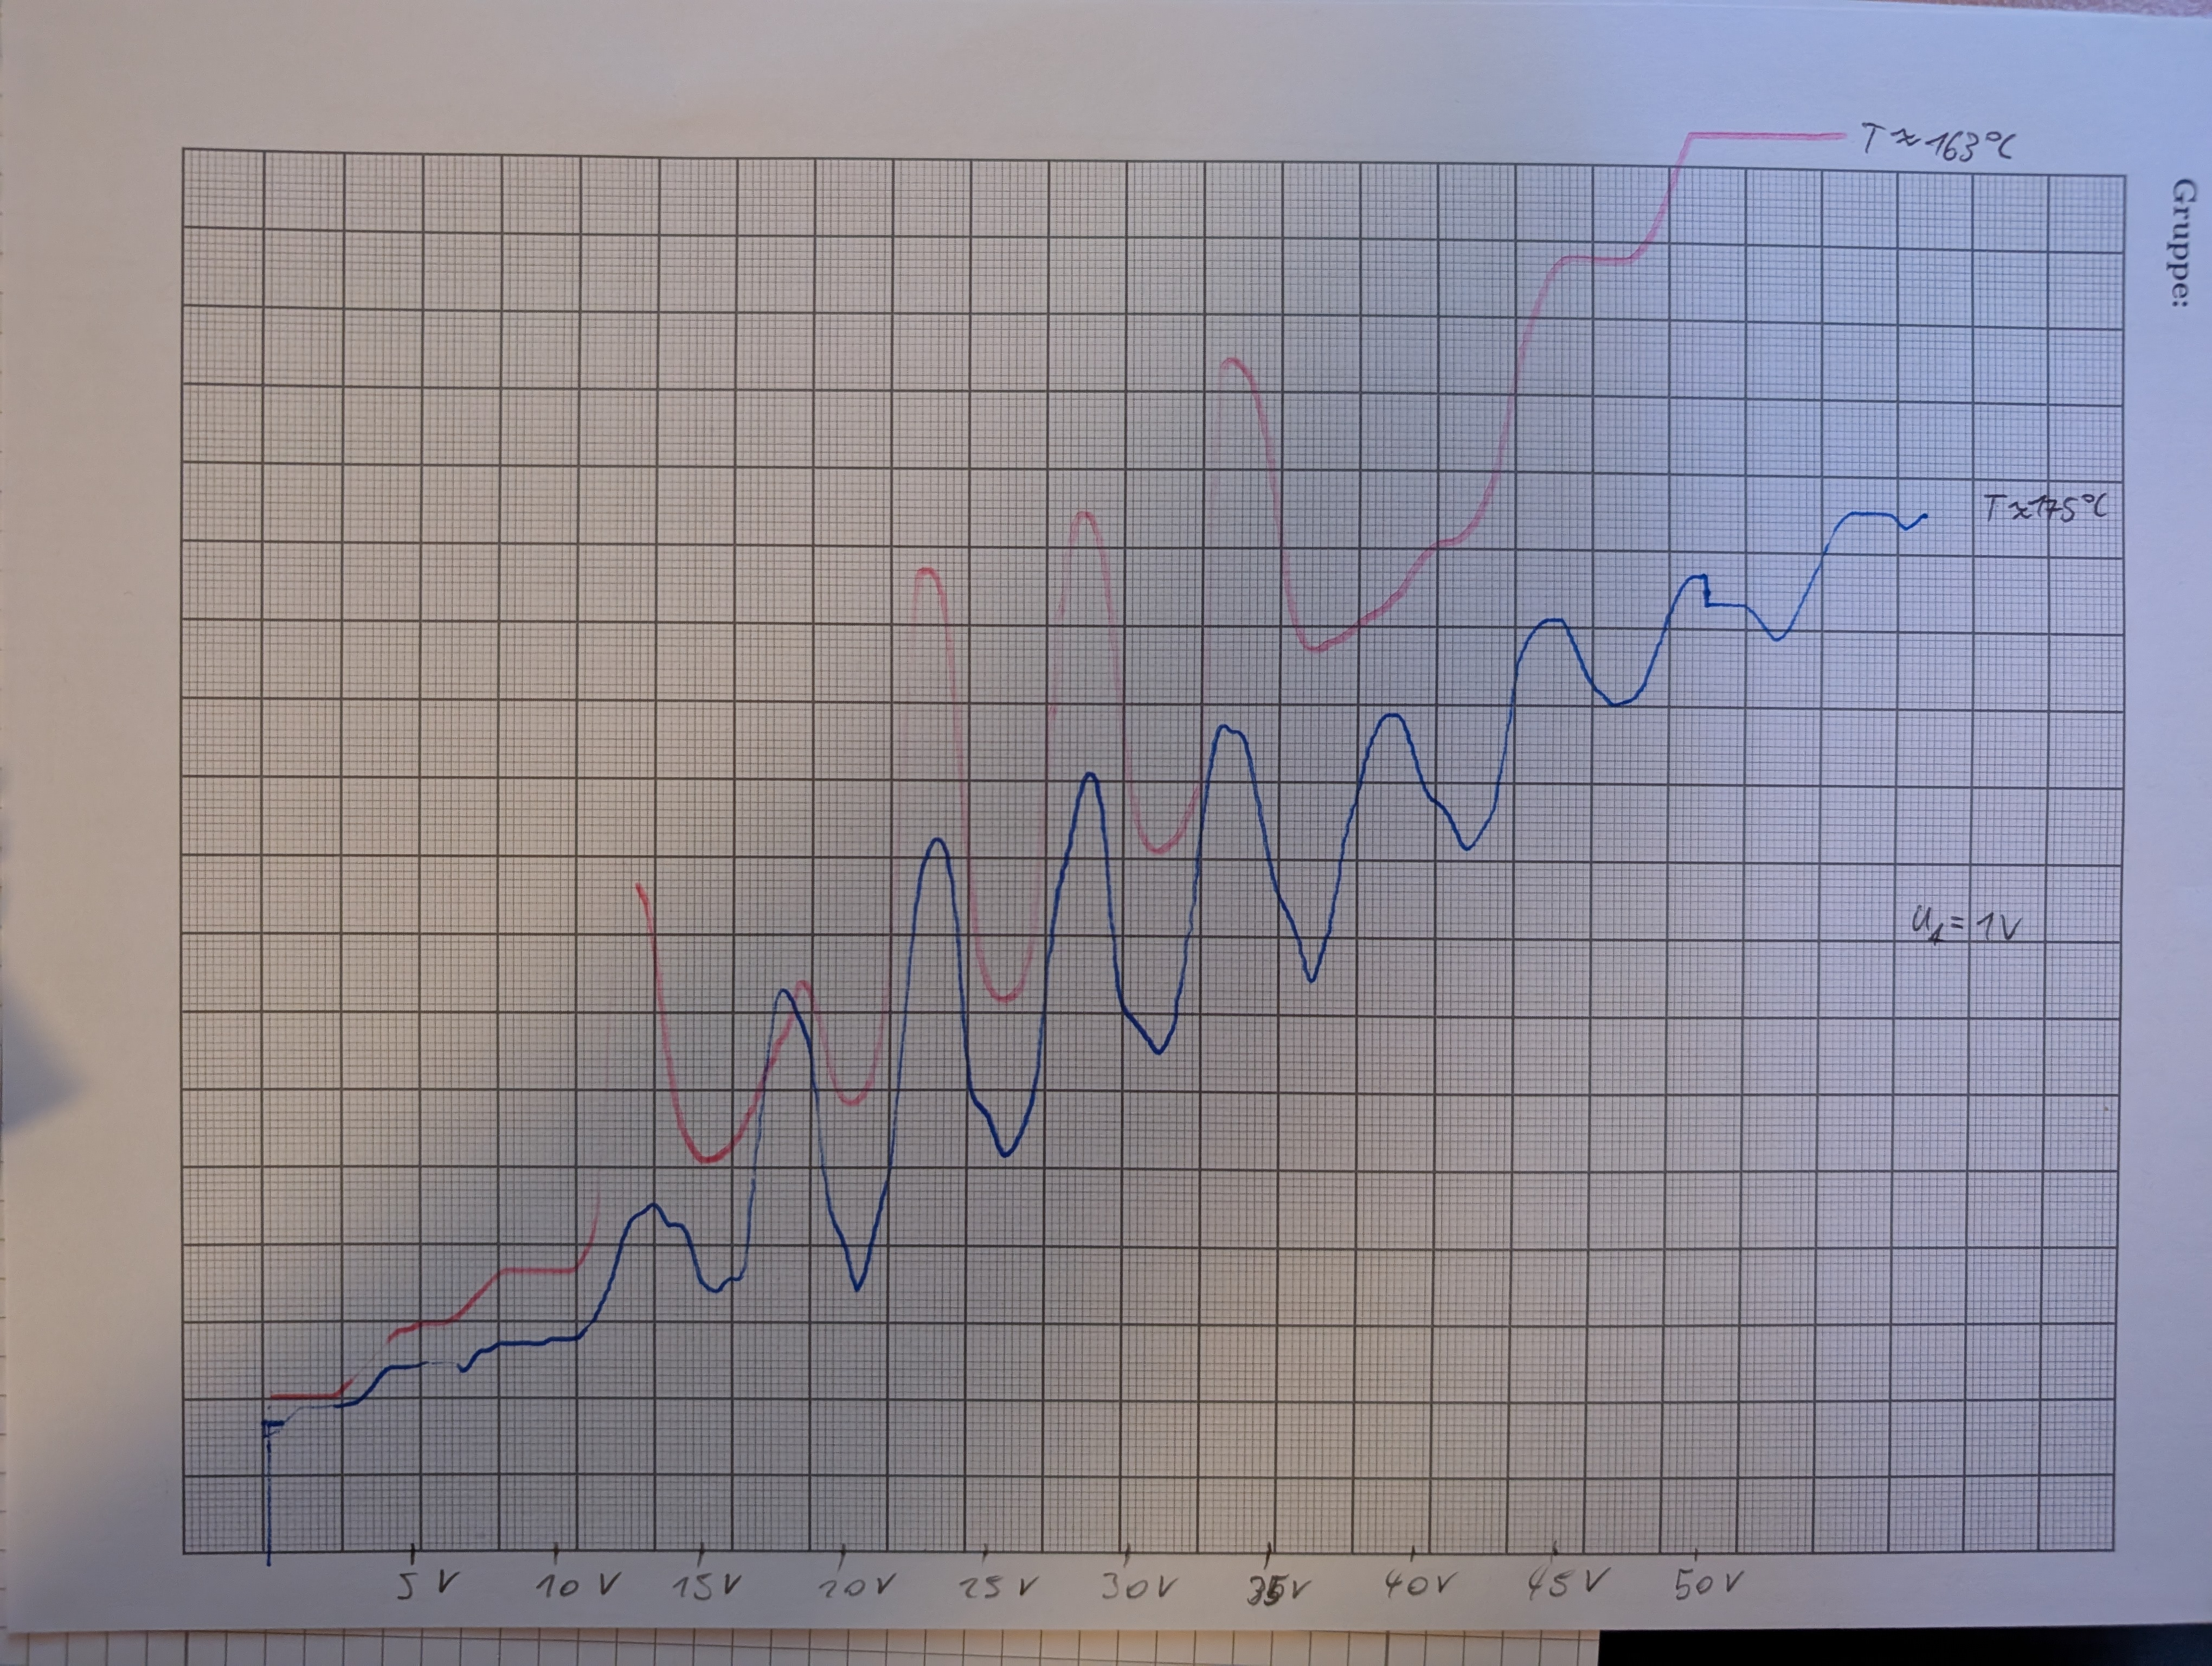
\includegraphics[width=0.85\linewidth]{Bilder/3.jpg}
  \caption{Franck-Hertz Kurven.}
  \label{fig:14}
\end{figure}
\noindent Relevant für die Auswertung sind die x-Werte der Maxima der
Frank-Hertz Kurven. Dementsprechend wird die blaue Kurve zur Auswertung 
herrangezogen, da bei dieser die Maxima deutlicher vorligen. Die x-Werte des
n-ten Maximums sind Tabelle \autoref{tab:12} zu entnehmen. 
\begin{table}[H]
  \centering
  \caption{Mittlere Freie Weglängen.}
  \label{tab:12}
  \begin{tblr}{
      colspec = {S S },
      row{1} = {guard, mode=math},}
         \toprule
         n & U_\text{gegen} \, / \, \unit{\volt} \\
         \midrule
          1 & 13.04\\
          2 & 17.39\\
          3 & 23.09\\
          4 & 28.39\\
          5 & 33.15\\
          6 & 41.71\\
          7 & 47.28\\
          8 & 49.59\\
          \bottomrule
  \end{tblr}
\end{table}

\begin{figure}[H]
  \centering
  \includegraphics[width=0.8\linewidth]{build/plot3.pdf}
  \caption{Maxima der blauen Franck-Hertz Kurve und Regression.}
  \label{fig:15}
\end{figure}
Die Parameter der linearen Ausgleichsrechnung sind
\begin{align}
  a =& \qty{5.5 (0.2)}{\volt} \\
  b =& \qty{6.7 (1)}{\volt},
\end{align}
wobei $a$ die Steigung und somit die durchschnittliche Beschleunigungsspannung
$U_\text{B} = \qty{5.5(0.2)}{\volt}$ angibt.
Aus $U_\text{B}$ kann mit 
\begin{equation}
  \lambda = \frac{\text{h} \cdot \text{c}}{U_\text{B} \cdot \text{e}}
\end{equation}
die Wellenlänge $\lambda$ bestimmt werden (siehe auch \autoref{eqn:lambda}).
Das ergibt eine Wellenlänge von 
\begin{equation}
  \lambda = \qty{2.25e-7} {\meter}
\end{equation}
Auch die Anregungsenergie lässt sich mit $U_\text{B}$ bestimmen:
\begin{equation}
  E_1 - E_0 = \qty{8.81e-19}{\volt}.
\end{equation}